\documentclass[
	twoside,
%	draft,
	fontsize=12pt,
	headsepline,
	cleardoublepage=empty,
	numbers=noenddot,
	bibliography=totoc,
]{scrbook}
%\clubpenalty = 10000 % schliesst Schusterjungen aus
%\widowpenalty = 10000 \displaywidowpenalty = 10000% schliesst Hurenkinder aus
\usepackage{ks}
\usepackage[onehalfspacing]{setspace}
\usepackage{todonotes}
\usepackage[]{algorithm2e}

% customize name, title, ...
\renewcommand{\thesisAuthor}{Mark Ugarov}
\renewcommand{\thesisTitle}{BBXYamlJava}
\renewcommand{\thesisDate}{Bielefeld, Decempber 2015}
\renewcommand{\thesisType}{Project report}
\renewcommand{\thesisCourse}{Cloudcomputing in bioinformatics }
\renewcommand{\thesisSupervisor}{Dr. Alexander Sczyrba  \\Dipl.-Inform. Jan Krüger  \\Peter Belmann}

\newcommand{\code}[1]{\texttt{#1}}

\begin{document}
\pagenumbering{gobble}
\begin{titlepage}
\fontfamily{phv}
\fontseries{m}
\selectfont
\leftskip2em

\begin{minipage}[t]{0.4\textwidth}
\large \thesisType\\
\normalsize \thesisCourse
\end{minipage}
\hfill
\begin{minipage}[t]{0.4\textwidth}
\begin{flushright}
CeBiTec, University of Bielefeld\\
\end{flushright}
\end{minipage}

\vfill

{\fontfamily{phv}\fontseries{bc}\selectfont 
\Huge \thesisTitle
\begin{flushright}
\Large \thesisAuthor
\end{flushright}
}

\vfill

\normalsize
\begin{minipage}[t]{5em}
\end{minipage}
\begin{minipage}[t]{0.5\textwidth}
\end{minipage}

\begin{minipage}[t]{5em}
Lecturers:\quad
\end{minipage}
\begin{minipage}[t]{0.5\textwidth}
\thesisSupervisor
\end{minipage}




\vfill

\thesisDate
\hfill

% enlarge page by 2 lines
\enlargethispage{2\baselineskip}

\end{titlepage}

\tableofcontents

\clearpage
\pagenumbering{arabic}


\chapter{Abstract and Basics}

BBXYamlJava is an extendible project trying to provide easy methods for parsing data used for bioboxes between an abstract data format and files (e.g. biobox.yaml - files) for maven projects. Thus it's not only necessary to implement an abstract data structure and the parsers but also to feature to go in depth of those structures with simple methods after parsing in from a file (what will be called Flatteners) or before parsing out into a file (which I described as Generators). 

In addition the implementation contains interfaces so the core (means the parsers themselves) can be left unchanged if the project is extended by new types of data. \\
The first attempt was to create all methods and classes to parse a list of assemblers out of a file, updating from a server. The second was to create a biobox.yaml - file for bioboxes with simple commands. To test the flexibility I also implemented a data structure for evaluation of assemblers.

This project report will include some figures giving you an overview of the implementation. Only public methods will be shown and the return type is not shown as long it is described by the name of the method or a equivalent set-method exists. Also some names of classes and methods will be bold: A user will not need to invoke any other classes or methods to successfully parse from or into a file with this project (excluding specific cases).

This project \cite{BBXYamlJava} was implemented as a maven project using netbeans \cite{Netbeans} including an ObjectMapper \cite{ObjectMapper} as a dependency. Originally this was part of a bigger project named BOCCS \cite{BOCCS} which was an attempt to make a GUI to run bioboxes \cite{BioBoxes} on a network.\\
All graphical elements where generated by using UMLet \cite{Umlet}. 

\chapter{Implementation}

This chapter describes crucial elements of the implementation and contains hints about potential further expansions. You may consider to have a look at figure \ref{fig:fullStructure} or at fullStructure.png in directory images while reading. Some important constants are stored in an abstract class \code{yamlparse.Constants} not shown in the figure. Elements involved in parsing from a file into a data structure are coloured green while elements involved in parsing from a data structure into a file are coloured cyan. Classes belonging to the data structure to parse to or from aregrey. The grey backlayers could be considered \emph{levels} or \emph{column}. Every further attempts to integrate new types of data to parse from or to a file should implement at least one entry in every column. 

\begin{figure}[h]
	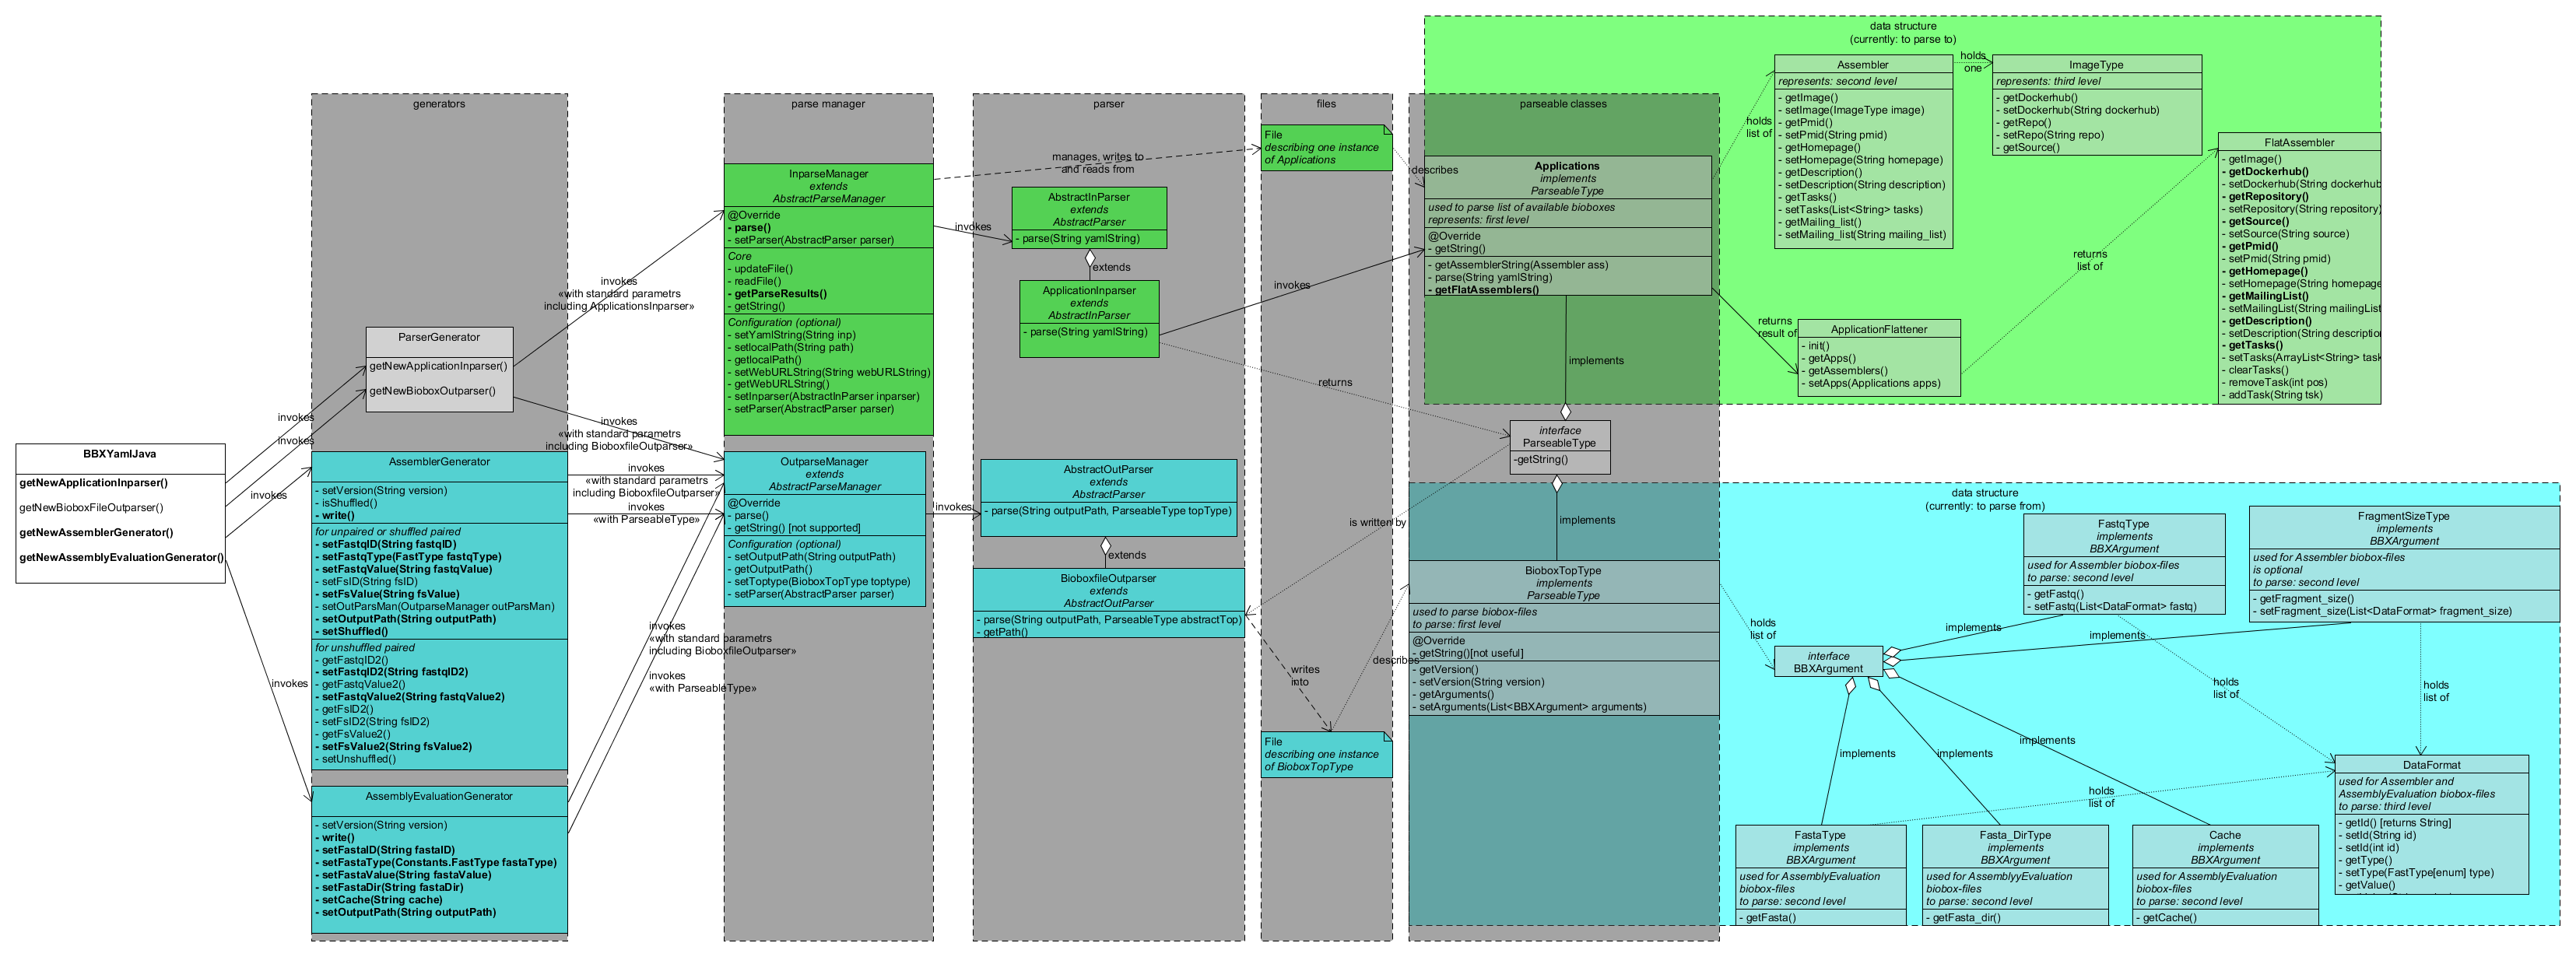
\includegraphics[scale=0.18, angle=90]{images/fullStructure.png}
	\label{fig:fullStructure}
	\caption{An overview of the full structure of the BBXYamlJava-Project. Since this is very tiny you may choose to have a look at the image in images/fullStructure.png}
\end{figure}

\section{Basics of parsing}
\label{sec:basicParsing}
The project uses an \code{ObjectMapper} (see more by exploring\\ \code{com.fasterxml.jackson.databind.ObjectMapper}) with a \code{YamlFactory} (see  \code{com.fasterxml.jackson.dataformat.yaml.YAMLFactory}) to parse implementation of the interface \code{ParseableType} (\code{yamlparse.datatypes.ParseableType}) into files or the other way round. This requires implementations of \code{ParseableType} as  a data structure representing several contents of a file. Currently there are two implementations of \code{ParseableType}: \code{BioboxTopType} (for biobox.yaml files, presently only to parse from a data structure into a file) and \code{Applications} (presently only to get a list of available bioboxes from a string into an abstract data format).

The actual parsing of instances of implementations of the \code{ParseableType} happens in extensions of the abstract data type \code{AbstractParser} which is extended into \code{AbstractInParser} and \code{AbstractOutParser} (see package \\ \code{yamlparse.parser.abstracts}). Originally all these classes where also ment to be interfaces, but JDK 1.7 seems to have a problem with interfaces of interfaces. Also I tried to implement only one \code{InParser} and one \code{OutParser} for all implementations of \code{ParseableType}, but this the \code{YamlFactory} is not able to process interfaces, so I had to create a \code{ApplicationsInparser} (to parse in instances of \code{Applications} from a string) and a \code{BioboxfileOutparser} (to parse out instances of \code{BioboxTopType} into a file). For further implementations: Every newly featured data type needs a similar parser itself unless there is a way to simplify the structure as described to only one \code{InParser} and one \code{OutParser} for all implementations of the interface \code{ParseableType} I don't know. 

These two components are all you need to parse: the parser and the underlying data structure. But the usability of this without features would be very bad so further classes are implemented to enhance it. 

\section{Enhance and simplify parsing for bioboxes}

To use these instances of \code{AbstractParser} some parameters are necessary: the path of the ouptut file or the content of the input file. To manage them I implemented an abstract class \code{AbstractParseManager} (which could have been an interface but interfaces do not allow constructors). Every extension of this class provides several methods to make parsing easier (see sections \ref{sec:inparse} and \ref{sec:outparse}). 

Trying to use these extensions still revealed some weaknesses: standard parameters had to be created every time and especially the construction of the \code{ParseableType} \code{BioboxTopType} didn't seem  to satisfy the needs of a simple usage. Thus I created group of classes I named \emph{Generators} which invoke an extension of \\ \code{AbstractParseManager} with standard parameters (without making it difficult to change them if necessary) and provide more adequate methods to create instances of \code{BioboxTopType} and write them into a file. See more about \code{AssemblerGenerator} and \code{AssemblyEvaluationGenerator} in section \ref{sec:outparse} or \code{ParserGenerator} in section \ref{sec:outparse} or in Figure \ref{fig:outparse}.

\begin{figure}[h]
	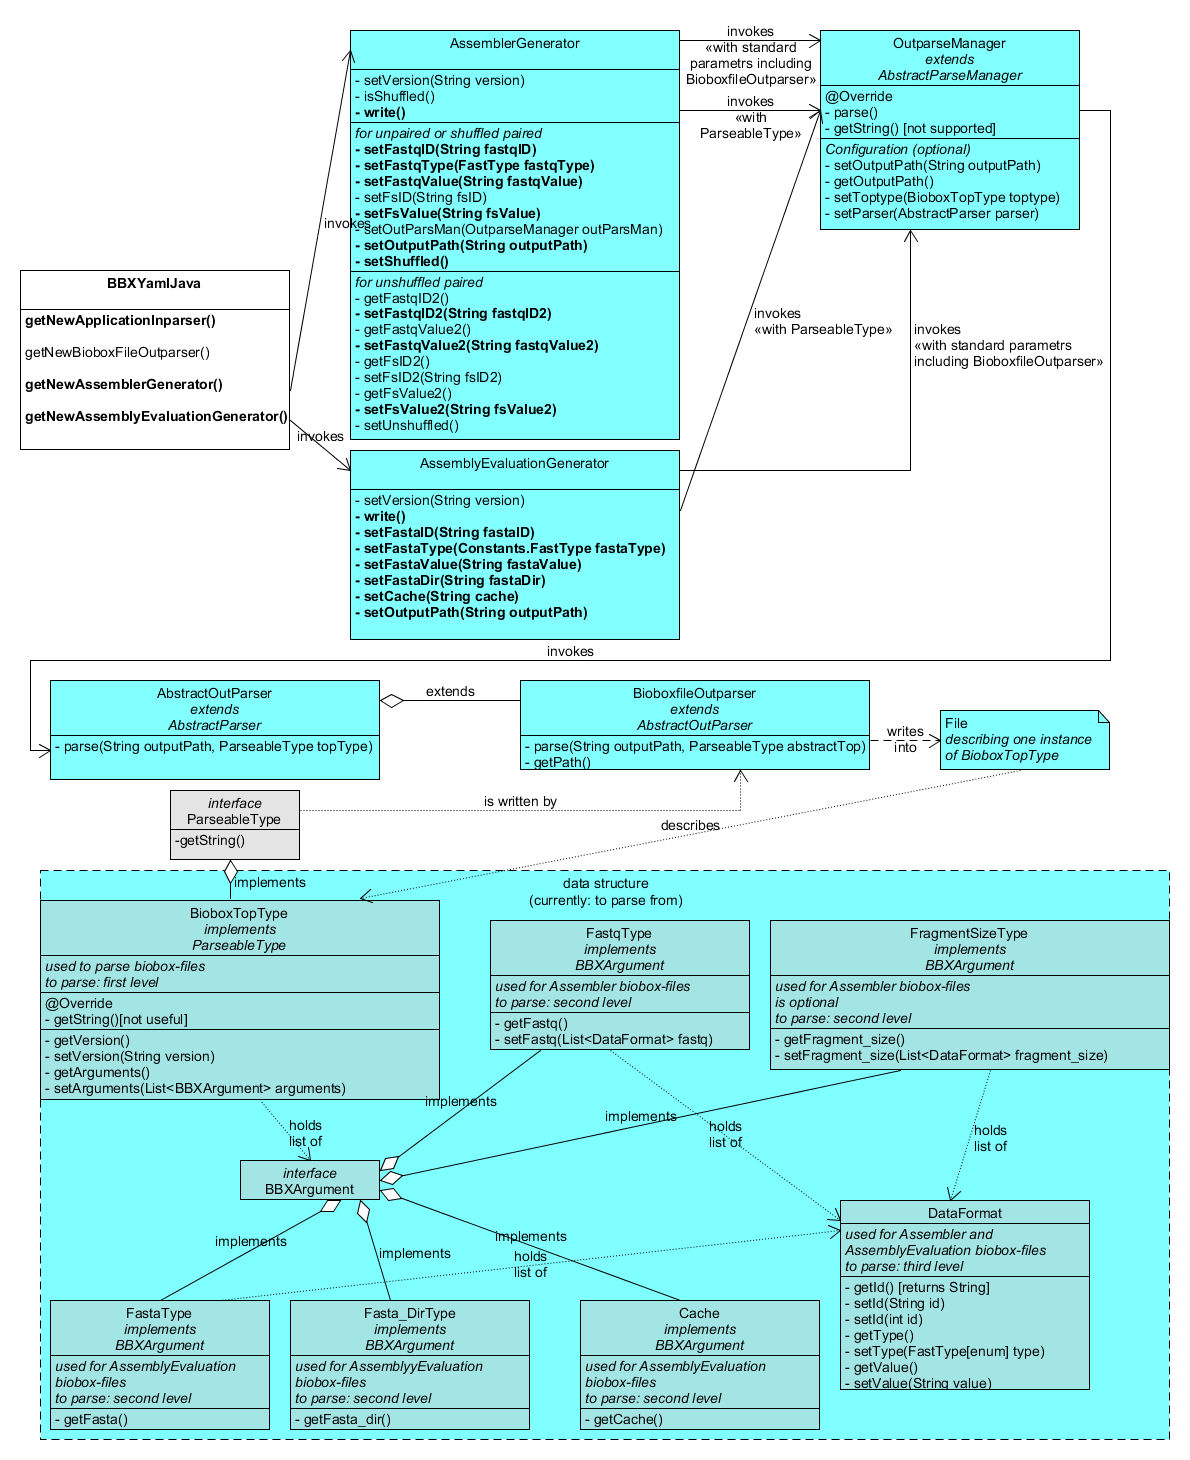
\includegraphics[scale=0.33]{images/outparse.png}
	\label{fig:outparse}
	\caption{An overview of the part of the project providing elements and methods to parse out yaml files for bioboxes in an easy way.}
\end{figure}

On the other hand I implemented a class \code{ApplicationFlattener} which creates a list of \code{FlatAssembler} to make it easy to get specific parameters out of an entry of \code{Applications}. Since instances of \code{Applications} have to be parsed before usage this class is not used in the \code{ParserGenerator} but in the \code{Applications} itself. Read more about \code{ApplicationFlattener} and \code{FlatAssembler} in section \ref{sec:inparse} or have a look at Figure \ref{fig:inparse}.

\begin{figure}[h]
	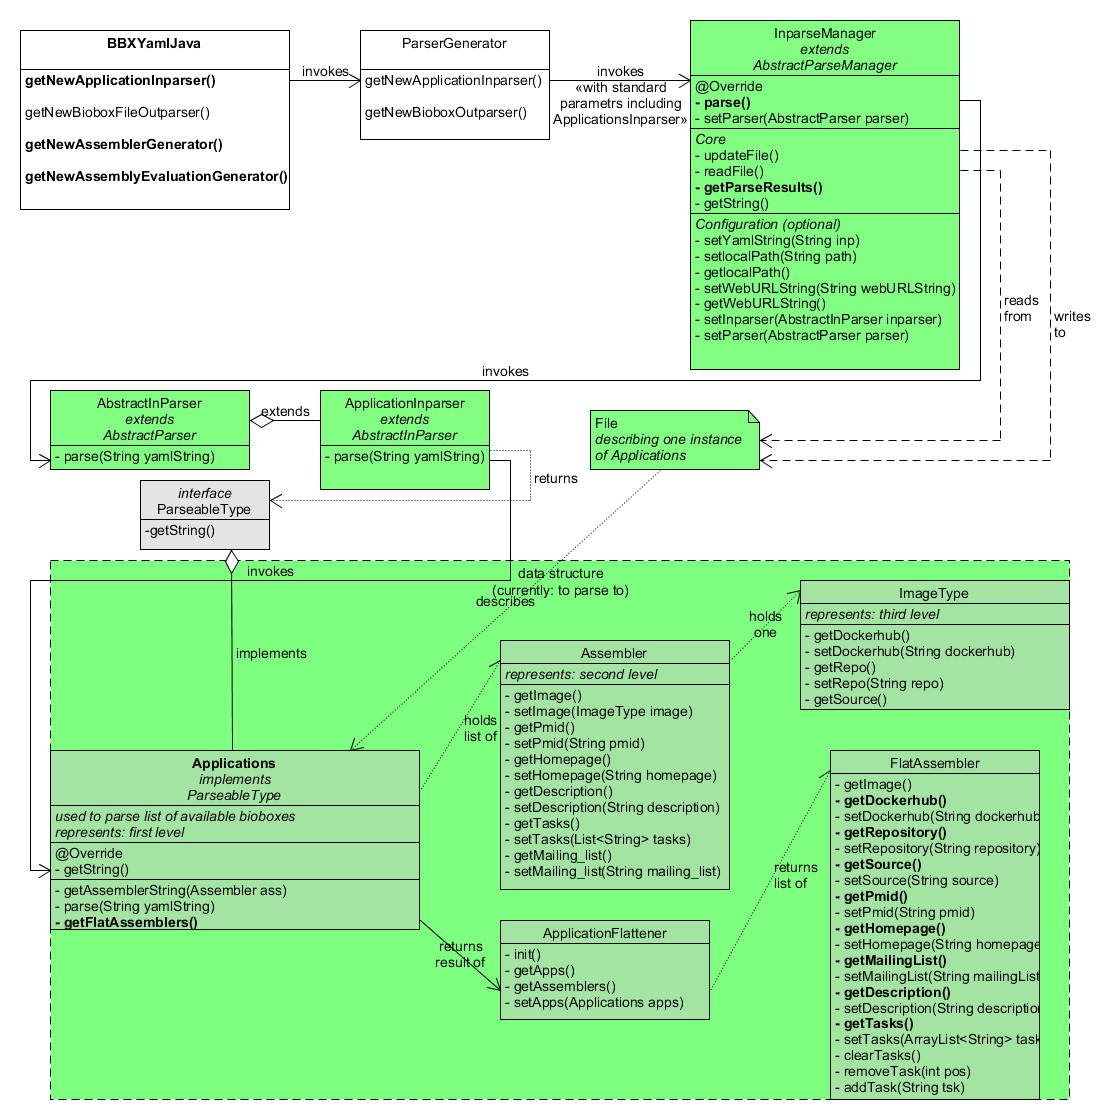
\includegraphics[scale=0.33]{images/inparse.png}
	\label{fig:inparse}
	\caption{An overview of the part of the project providing elements and methods to parse a data structure out of a file in an easy way.}
\end{figure}

Before jumping into the next chapter I want to mention two deviations:
As you can see the methods \code{getNewApplicationInparser()} and \\ \code{getNewBioboxFileOutparser()} do not return instance of \code{AbstractParser} but extensions of \code{AbstractParseManager} since I decided to name those methods in view of readability and intuition instead of clear structure. This seems to be confusing at first, but be sure that the parsing itself is much more comfortable as you can see in \ref{sec:outparse}. Feel free to use instances of \code{AbstractInParser} (e.g. \code{ApplicationInParser}) and \code{AbstractOutParser} (e.g. \code{BioboxfileOutparser}) for special needs.
Also I named generators based on their purposed type of \emph{biobox} if they are implemented for specific usage, e.g. \code{AssemblerGenerator} provides methods to write a \emph{yaml} file for bioboxes containing an assembler. In contrary the \code{ParserGenerator} has the more general purpose to invoke instances of \code{AbstractParseManager} without further additions. We will discuss differences in chapter~\ref{chap:usage}. 


\chapter{Usage}
\label{chap:usage}

For a good usability take a look at the main class \code{BBXYamlJava} in package \code{yamlparse}. Every method uses (or returns) an instance of a group of classes I called \emph{Generators}. The attempt is to invoke crucial classes (or methods) with standard parameters on one hand and make it easy to set crucial parameters on the other hand. 

Please note that there are two levels of Generators in this project:
\begin{itemize}
	\item The \code{ParserGenerator} only provides methods to invoke extensions of \\ \code{AbstractParseManager} (\code{InparseManager} or \code{OutparseManager)} with standard parameters (including an implementation of \code{AbstractParser}). Those are implemented for file management like to set paths (to read from or to write to), to download and so on. They are sufficient to parse from a file into an abstract data structure. 
	\item Other \emph{Generators} for usage of specific implementations of \code{ParseableType}. Those are currently implemented for instances of \code{BioboxTopType} with differentiations: \emph{bioboxes} containing assemblers do need other parameters than \emph{bioboxes} for assembly evaluation. Their purpose is to ease the process of setting parameters of \code{BioboxTopType} in a significant amount. There is no need for the user to call other methods than provided by these \emph{Generators} to generate a data type and write it into a file. 
\end{itemize}

Thus don't confuse about the classes AssemblerGenerator and Assembler:
An instance of \code{Assembler} holds values each describing a \emph{biobox} containing an assembler while an instance of \code{AssemblerGenerator} can write a \emph{yaml} file for the usage of the described assemblers. 

\section{Parsing an abstract data structure into a file}
\label{sec:outparse}
The current implementation only allows to parse out BioboxTopType, so this section will focus on this. If you want to apply your own data type please have a look at figure \ref{fig:fullStructure} and section \ref{sec:basicParsing}. 

Before parsing a new instance of BioboxTopType is needed. The project BBXYamlJava provides two ways to do so: Manually by the user or automatically by \emph{Generators}. In case you did not read the beginning of this chapter: There is no need to use other methods other than provided by the \code{AssemblerGenerator} to write a \emph{yaml} file for use with a \emph{biobox} containing an assembler and the same principle applies to \code{AssemblyEvaluationGenerator}. 

Those generators are a more comfortable way to create \emph{yaml} files than invoke a \code{ParseableType} and parse them with an extension of \code{AbstractOutParser} (like \code{BioboxfileOutparser}):
They hold the all parameters as a \code{ParseableType} (e.g \code{BioboxTopType}) with an usual number of entries would hold, but you can set parameters directly even if they have a higher level. 
E.g. you can set the \code{fastq} value by  \code{\#AssemblerGenerator().setFastqValue(String fastqValue)} instead of \code{((FastqType) \#BioboxTopType.getArguments().get(0)).getFastq() \\ .setValue(String value)}. 

After setting those parameters, the user can use the \code{write()} method to write it to the \code{outputPath}. 

By usage of \code{AssemblerGenerator} you will find an important field of type \code{boolean} named \code{shuffled} and another of type \code{Constants.FastType} called \code{fastqType}: You may know that there are two kind of reads which are \emph{paired} and \emph{unpaired}. The \emph{fastq} files of \emph{paired} reads may occur in two separate files (which means the sequences are \emph{unshuffled}) or alternating in one file (which means the sequences aren't \emph{shuffled} or might say \emph{unshuffled}). Make sure you choose the right setting for your needs.

\section{Parsing a file into an abstract data structure}
\label{sec:inparse}

To parse an existing file (or string) into an abstract data structure this project includes a class named \code{InparseManager}. If you choose to use this class with your own extension of \code{AbstractParser}, you have to set it as well as at least one of the following parameters: 
\begin{itemize}
	\item the string to parse from
	\item a path to a file containing the string
	\item an url directing to a file and the path where to save it
\end{itemize}

If you choose the first one, consider to use extensions of \code{AbstractInparser} like \code{ApplicationInparser} instead.

Since the only current usage is to parse an instance of \code{Applications} (which contains a list of \code{Assembler} the following will describe how to use the instance you get by calling \code{\#BBXYamlJava.getNewApplicationInparser()}.

This instance has a default url where to download a file containing all bioboxes currently available \cite{AssemblerList} at default. Of course you can set your own url in case you want to download any other file.

The following is optional before invoking \code{parse()}: By invoking the method \\ \code{updateFile()} the file will be downloaded to a local path (which is the working directory at default) and the yaml string will be set to its content. 
If you have your own file instead, you may also set the local path and invoke \code{readFile()}. You can also set the yaml string manually as mentioned. 

If at least one parameter is set as described above, you can invoke the method \code{parse()}. This will read from the local file if the yaml string is not set yet and download the file if the local file is empty. 

After parsing you can get the result by \code{getParseResults()} which returns a \\ \code{ParseableType} you have to cast to \code{Applications} which again is a tree like data structure. Thus it seems very unhandy use that class. A more comfortable solution might be to invoke \code{\#Applications.getFlatAssemblers()} which returns a \code{ArrayList} of \code{FlatAssembler}. An instance of class \code{FlatAssembler} contains the same paramters as parsed instance of \code{Assembler}, but instead of tree like its method only return strings and \code{ArrayLists} of strings.

As you can see some results have to be cast. This is not very satisfying, but I did not find another solution supporting the structure of the project which I chose to be easy to extend. 

\printbibliography


%%

\thispagestyle{empty}

\end{document}
